\documentclass{article}
\usepackage[utf8]{inputenc}
\usepackage{graphicx}


\title{Gestione di Reti 21-22}
\author{Ambra Manattini}
\date{February 2022}

\begin{document}

\maketitle

\tableofcontents
\newpage

\section{Ethernet}
\subsection{Topologie}
\subsubsection{Cavo Ether}
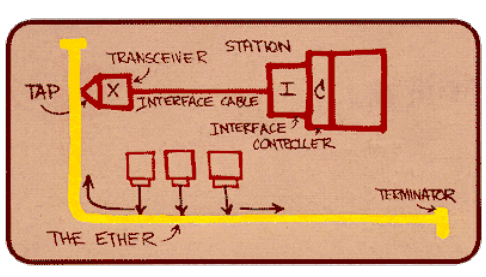
\includegraphics[]{ethernet.png}

Inizialmente si ha un cavo (the ether) al quale vengono collegate le varie stazioni (facendo proprio buchi nel filo).
Le varie stazioni sono caratterizzate da controller e interface.

\textbf{Interfaccia}: traduce quello che il controller(?) può capire allo standard ethernet.
Le informazioni sono divise in \textbf{pacchetti}, vengono mandate da sorgente e destinazione (locale). 
\par Si creano diversi problemi di interferenza visto che i pacchetti vengono mandati in entrambe le direzioni del cavo e praticamente a tutti
\subsubsection{Topologia Bus e Stella}
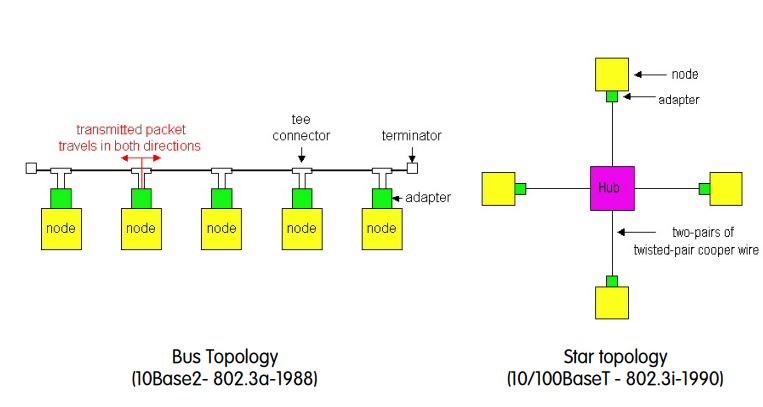
\includegraphics[width=\linewidth]{2.png}
Abbastanza simile alla precedente, le stazioni sono connesse al cavo tramite un connettore (\textit{tee connector}, i pacchetti viaggiano ancora in entrambe le direzioni

\par \textbf{Topologia a Stella}: non c'è più il coassiale, ma il doppino; che trasmette non da più fastidio a chi riceve, non si usa più lo stesso cavo per mandare e ricevere, non sono più connesso direttamente alle altre stazioni, tutto il traffico passa dallo switch.

\subsection{Tecnologia}
\subsubsection{Full-duplex}
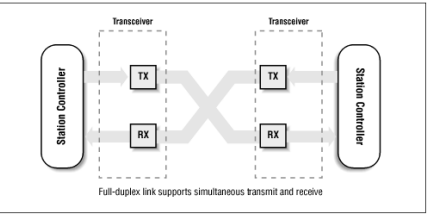
\includegraphics[]{3.png}

\par Prima ethernet trasmetteva in half-duplex (o parlo o ascolto), adesso la tecnologia è full-duplex (le stazioni possono simultaneamente inviare e riceve) hanno fisicamente diviso invio e ricezione

\subsubsection{PoE (Power over Ethernet}
\par corrente che passa dal cavo di rete, utilizzato per dispositivi che hanno bisogno di poca elettricità (es. access point)


\subsection{Ethernet framing}
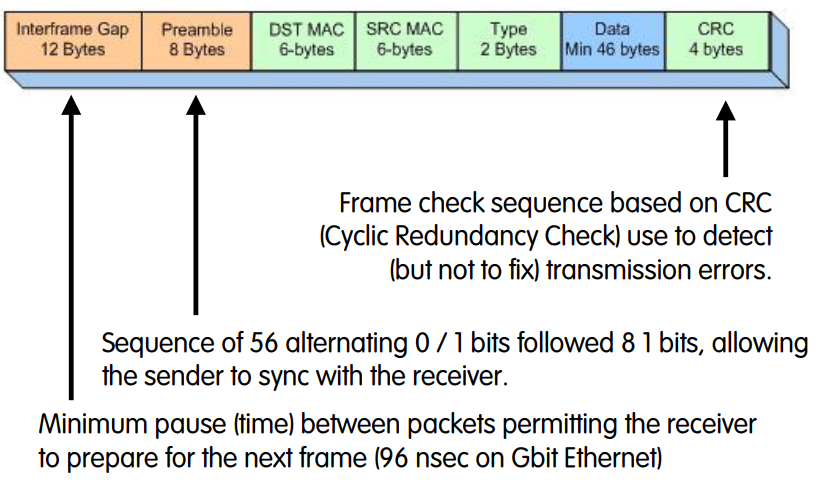
\includegraphics[width=\linewidth]{4.png}
Livello 2 dello stack
Per i pacchetti ethernet non c'è la lunghezza, si riconoscono per i separatori all'inizio e alla fine
Gli indirizzi sono tipicamente della scheda di rete del source e destination.
Lunghezza minima 60bytes. 


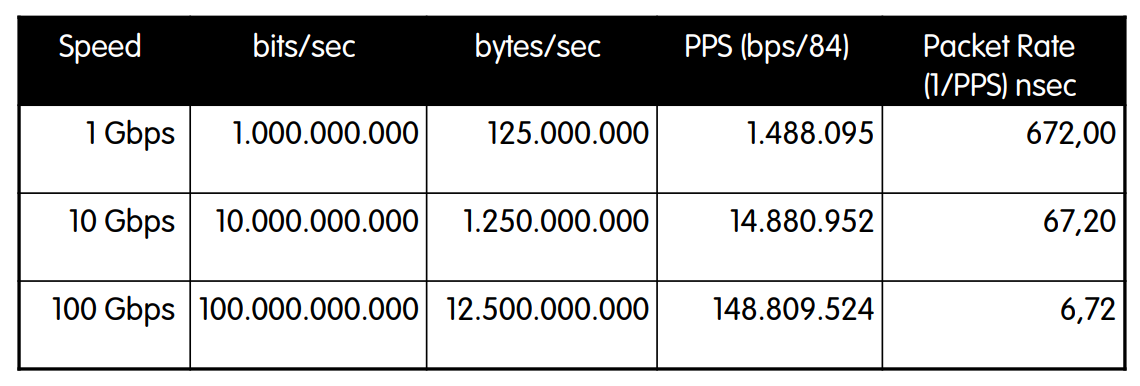
\includegraphics[width=\linewidth]{5.png}

\subsection{Ethernet switches}
Le stazioni ethernet comunicano sempre direttamente, gli switch sono invisibili, non modificano il pacchetto.
Gli switch non hanno bisogno di configurazione, lavorano analizzando il traffico di rete.

Quando una stazione si connette avvisa della sua presenza tramite un frame; allo switch arriva il frame e si annota l'indirizzo associato alla porta nella \textbf{Forwarding Table}.
Per ogni porta ci possono essere più mac address.

Il traffico è inviato in base all'indirizzo di destinazione:
\begin{enumerate}
    \item Quando viene ricevuto un frame il MAC viene cercato nella FT
    \item Se viene trovato viene mandato nella porta associata all'indirizzo
    \begin{enumerate}
        \item Se non viene trovato viene mandato su tutte le porte tranne quella da cui è arrivato
    \end{enumerate}
\end{enumerate}

\par\textit{\textbf{scartare}: attività volontaria, decido di non gestire il pacchetto\\
\textbf{droppare}: non riesco a gestire il pacchetto}\\
\par \textbf{VLAN}\\
%boh non ho molto capito
I tag VLAN sono invisibili, li vedono solo gli switch, serve per mandare i pacchetti in broadcast sulle VLAN

\par La robustezza si fa tramite la ridondanza; devo far sì che ci sia più di un cammino verso dei punti critici di una rete, così in caso un cammino non sia disponibile il servizio rimane attivo\\
metto più cavi tra gli switch ( ad es i server importanti hanno tutto raddoppiato)

\section{Introduzione}
\subsection{Managed Objects}
\par \textbf{Management Information Base}
%xd

\par \textbf{Manager/Agent Paradigm}


L'\textbf{agent} è un software che accede alla risorsa reale, riceve dal manager una richiesta,la gestisce e trasmette la risposta.
Invia notifiche sui cambiamenti importanti dello stato.
Protegge dagli accessi non autorizzati.
%elenco ?

Il \textbf{manager} esercita il controllo.
Inizia le operazioni di configurazione.
Riceve i messaggi dagli agenti e li passa alle appropriate applicazioni.

\subsection{Services and Protocols}
\par \textbf{Definizioni}

Quattro primitive o famiglie di primitive; quando invio la richiesta, lato mittente (client) : \textbf{request}.

quando è in viaggio si parla di \textbf{indication}

\textbf{risposta} e \textbf{conferma} per la parte di risposta 

quando faccio una richiesta e passa nella rete, il contenuto è lo stesso, ma il pacchetto viene modificato.
a livello di pacchetto ci possono essere delle modifiche, a livello di servizio viene alterato, ogni volta che passa da un host viene aggiunto qualcosa

\subsection{Livelli}
Quando partono le richieste passano da più livelli. I livelli adiacenti parlano tra loro

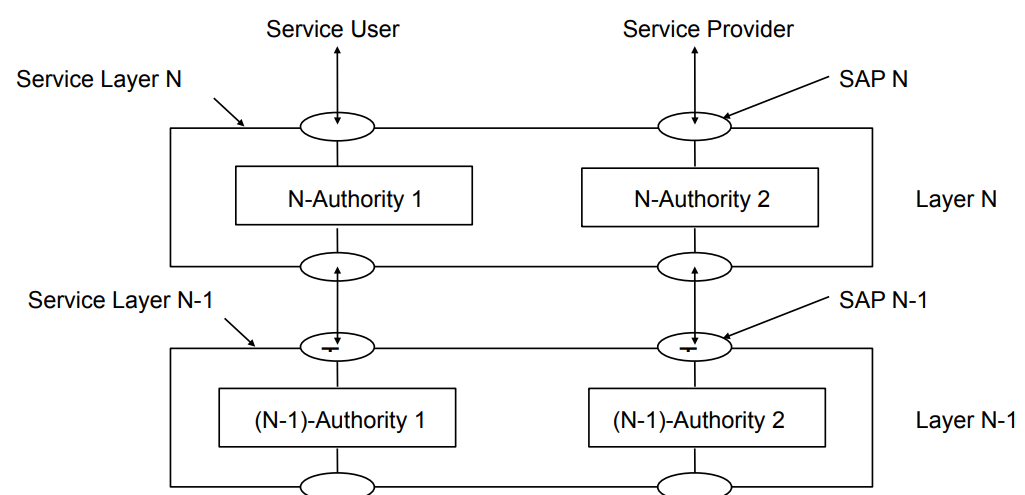
\includegraphics[width=\linewidth]{6.png}

\par \textbf{Time diagrams}

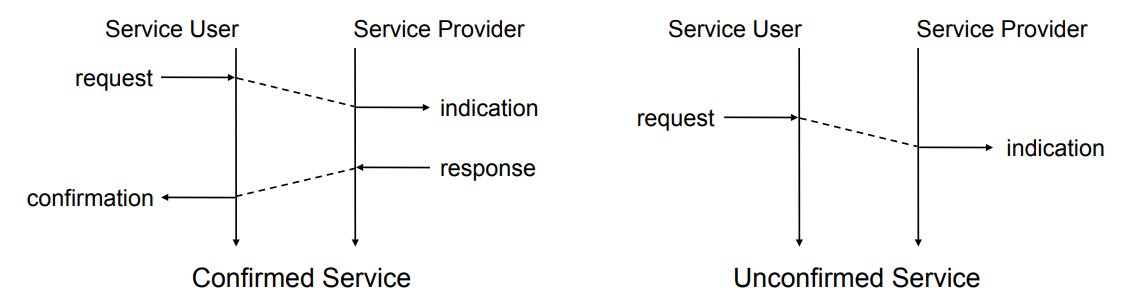
\includegraphics[width=\linewidth]{7.png}
I servizi possono essere confermati o non confermati
\par \textbf{ASN1}
Meccanismo per trasportare le informazioni tra client e server scambio di informazioni tra macchine con hardware diverso, indipendente dai linguaggi di programmazione (\textit{language neutral}), il sistema di codifica è negoziato all'inizio dello scambio dei dati
\par \textbf{Abstract Syntax and Tranfer Syntax}
%immagine dell'ASN ma non lo chiede all'esame
ASN definsice una sintassi astratta standardizzata

\section{Protocolli di Gestione}

\end{document}
